\section{Task 4: Simulink and Simulation}
\FloatBarrier % Now figures cannot float above section title

\subsection{Simulink}
Figure \ref{F 5.1} shows a schematic of Simulink.
\begin{figure}[htp]
    \centering
    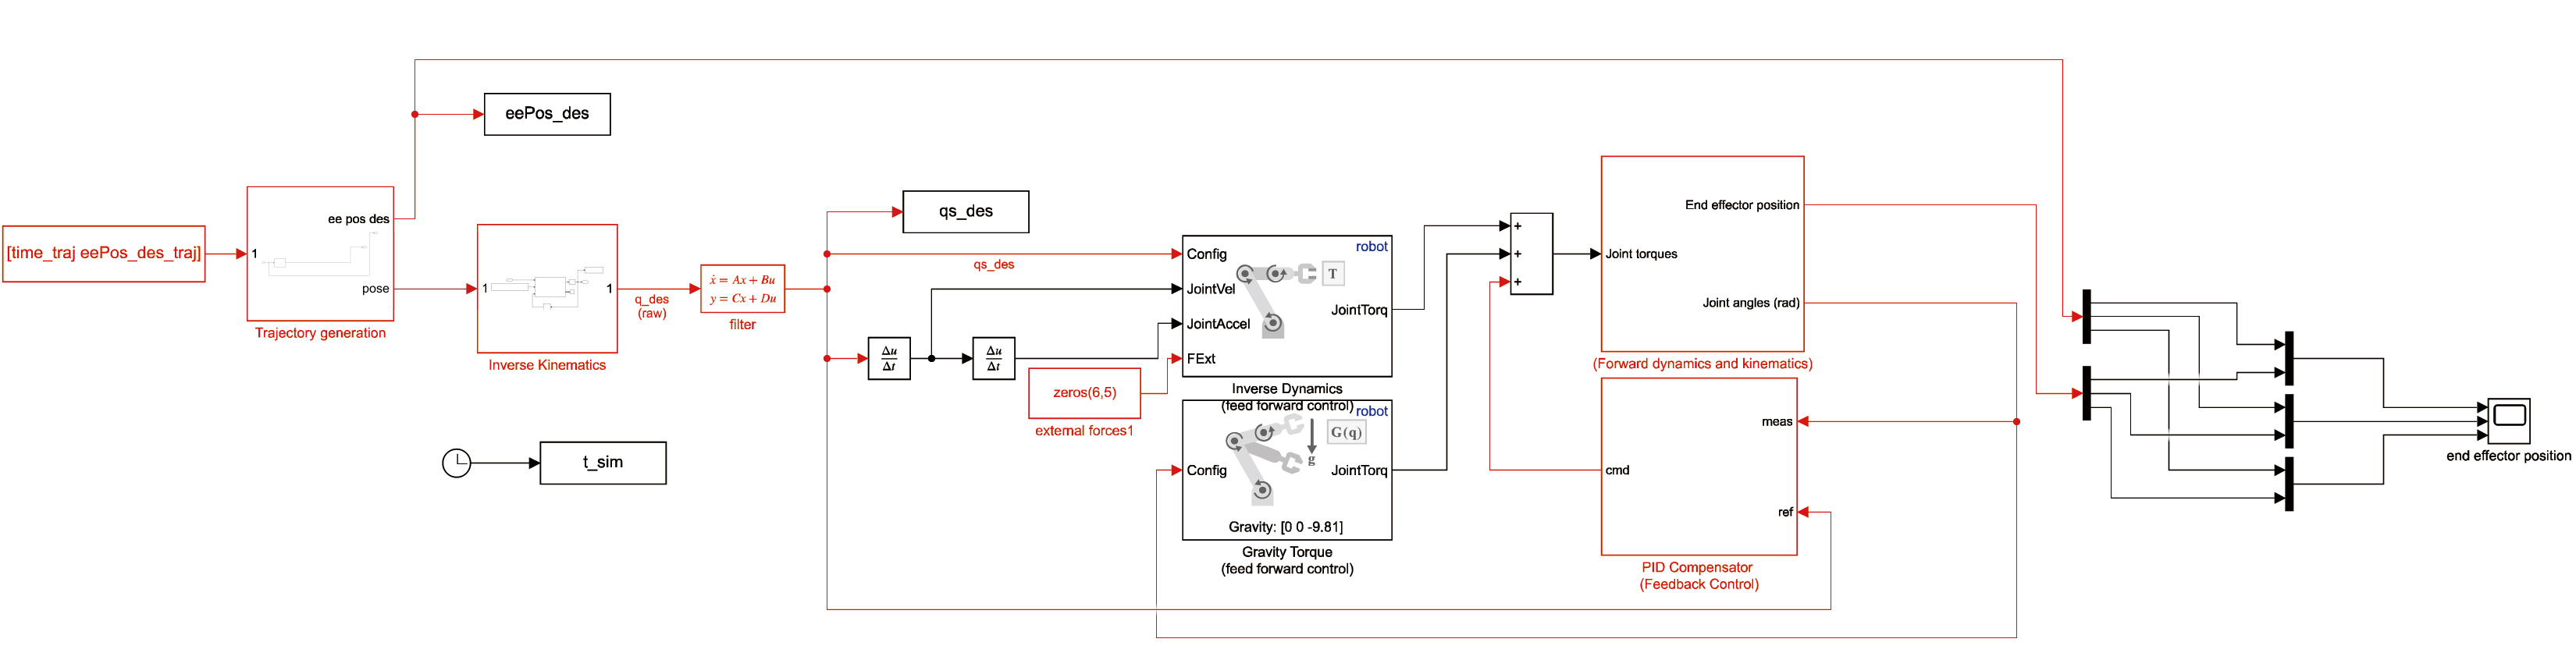
\includegraphics[width=17cm]{./fig/sim.jpg}
    \caption{The Simulink}
    \label{F 5.1}
\end{figure}

\subsubsection*{Tidy of the model}
To ensure aesthetic appeal, a modular design approach was adopted, where different modules represent different functionalities, thereby making the overall model's operation flow appear clear and concise.

\subsubsection*{Trajectory generation}

\begin{figure}[htp]
    \centering
    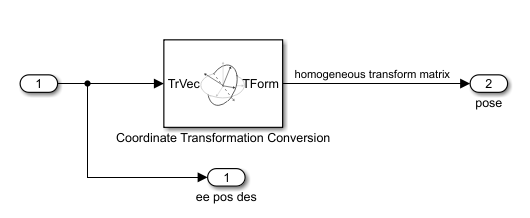
\includegraphics[width=10cm]{./fig/traj.png}
    \caption{Trajectory generation schematic}
    \label{F 5.2}
\end{figure}

We first calculate the path coordinate points and time series from the code, and use them as input parameters for trajectory calculation. Through trajectory calculation as shown in \autoref{F 5.2}, we can obtain the expected end-effector position and obtain motion trajectory data applicable to each point after coordinate transformation (which records the three-dimensional coordinate points of the path every 0.01 seconds).

\begin{figure}[htbp]
	\centering
	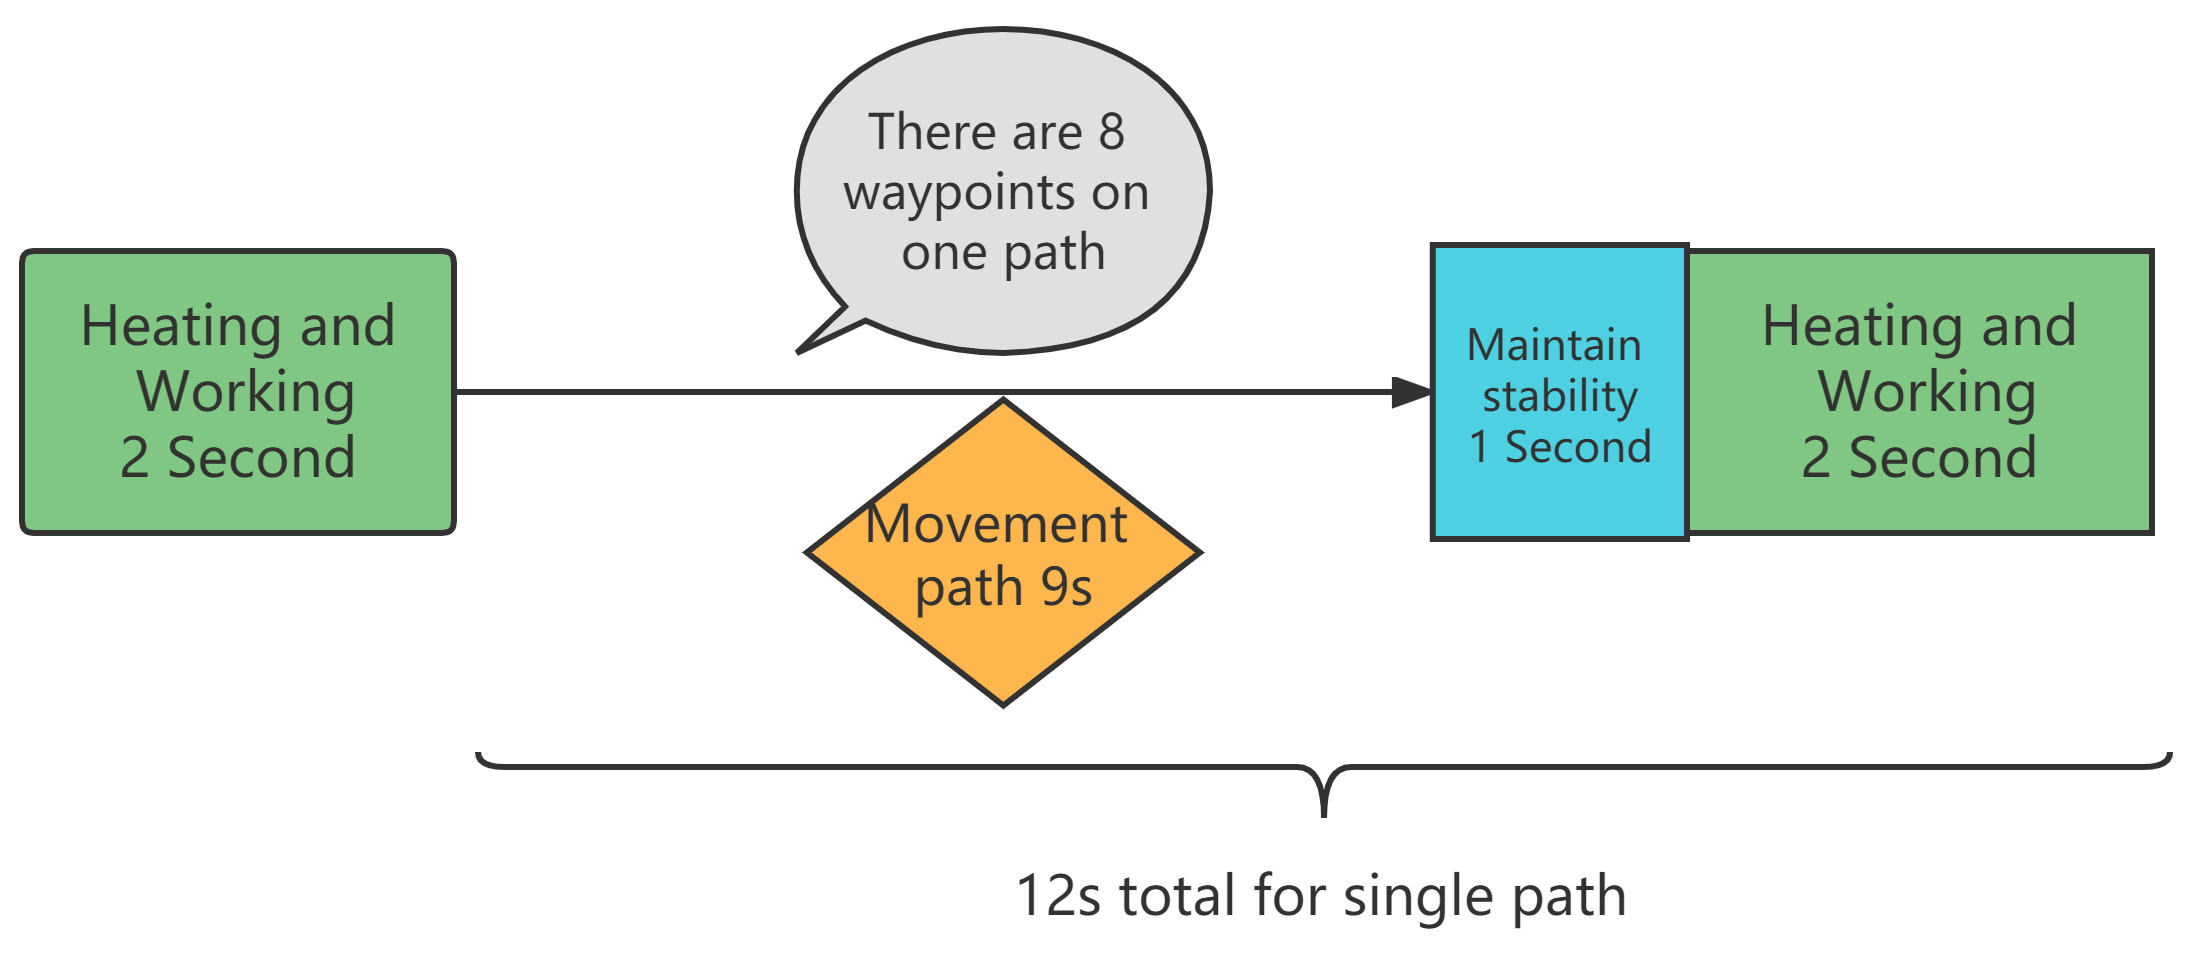
\includegraphics[width=10cm]{./fig/siwei.png}
	\caption{Flowcgart of trajectory generation }
	\label{F 5.3}
\end{figure}

\autoref{F 5.3} is a flowchart of the process we use to compute the trajectory of the robot's end effector position. First, we divide the rectangle required for the task into four line segments. For each line segment, we divide it into 9 equally long segments, and expect the robot to take 9 seconds to move along it. After that, the robot needs to spend 1 second for stabilization, followed by 2 seconds of welding work at the work point. Totally, it takes 48 seconds for the robot to complete the welding task. To account for this, we designed a simulation time of 48 seconds. 

\subsubsection*{Inverse kinematics}

In the inverse kinematics module, we use the expected end-effector position as input, as shown in \autoref{F 5.4}, and calculate the expected joint angles using inverse kinematics. The output is a matrix containing time-series data, which records the rotation angles of different joints of the robotic arm every 0.01 seconds.
\begin{figure}[htbp]
	\centering
	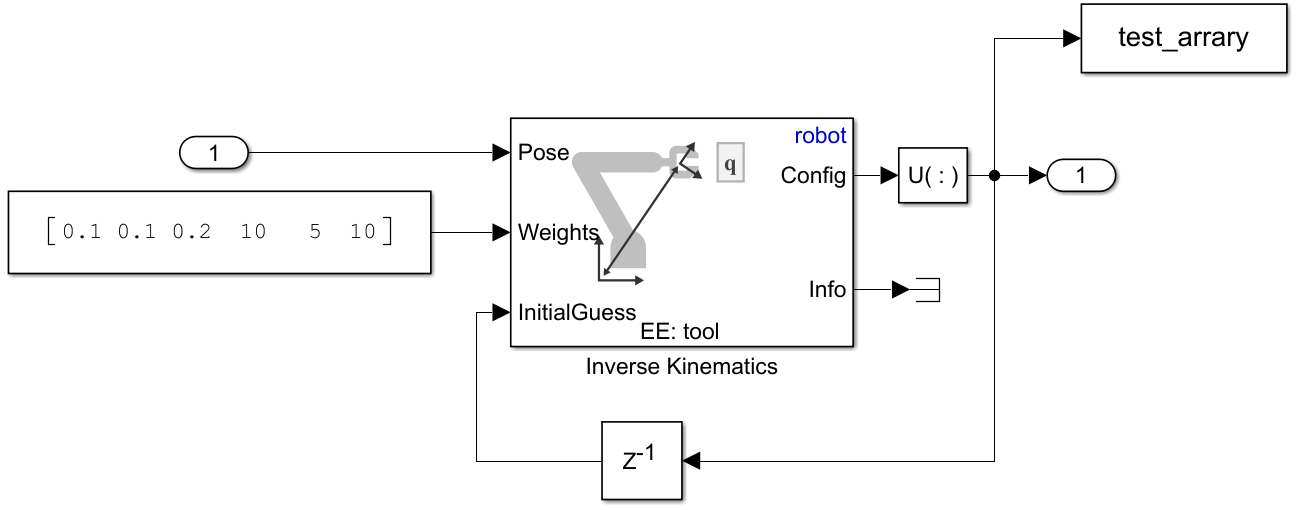
\includegraphics[width=8cm]{./fig/IK.png}
	\caption{Inverse kinematics}
	\label{F 5.4}
\end{figure}

\subsubsection*{Inverse dynamics}

Inverse dynamics is to calculate the forces or torques that are required to produce a desired motion of a robotic system. The technique involves using the system's equations of motion to determine the forces or torques required to generate a desired trajectory or motion. As shown in \autoref{F 5.5}, the input parameter in this part is the coordinate data of each sampling point calculated by the inverse kinematics. By weighting and differentiating the data, the required angular velocity and angular acceleration can be obtained. Then, the obtained data is imported into the inverse dynamics module for calculation, and the result is the torque required for each joint at each sampling point.

\begin{figure}[htbp]
	\centering
	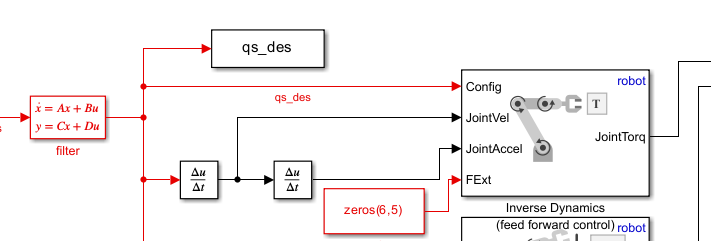
\includegraphics[width=10cm]{./fig/ID.png}
	\caption{Inverse dynamics}
	\label{F 5.5}
\end{figure}

\subsubsection*{Gravity}


In this part, the torque generated by gravity is added as a vector to the torque required by each joint calculated by the inverse dynamics module, and the combined torque vector is passed to the next module to simulate the deviation that may occur in the actual robot arm. The process is shown in \autoref{F 5.6}.


\begin{figure}[htbp]
	\centering
	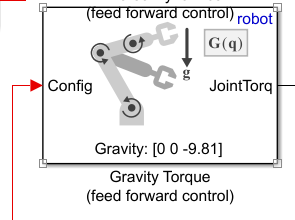
\includegraphics[width=5cm]{./fig/G.png}
	\caption{Gravity part}
	\label{F 5.6}
\end{figure}


\subsubsection*{Forward dynamics and kinematics}


\autoref{F 5.7} shows the forward kinematics and dynamics module, in which the actual position and orientation of the end-effector can be calculated based on the actual joint angles obtained by considering the different torques inputted to each joint.

\begin{figure}[htbp]
	\centering
	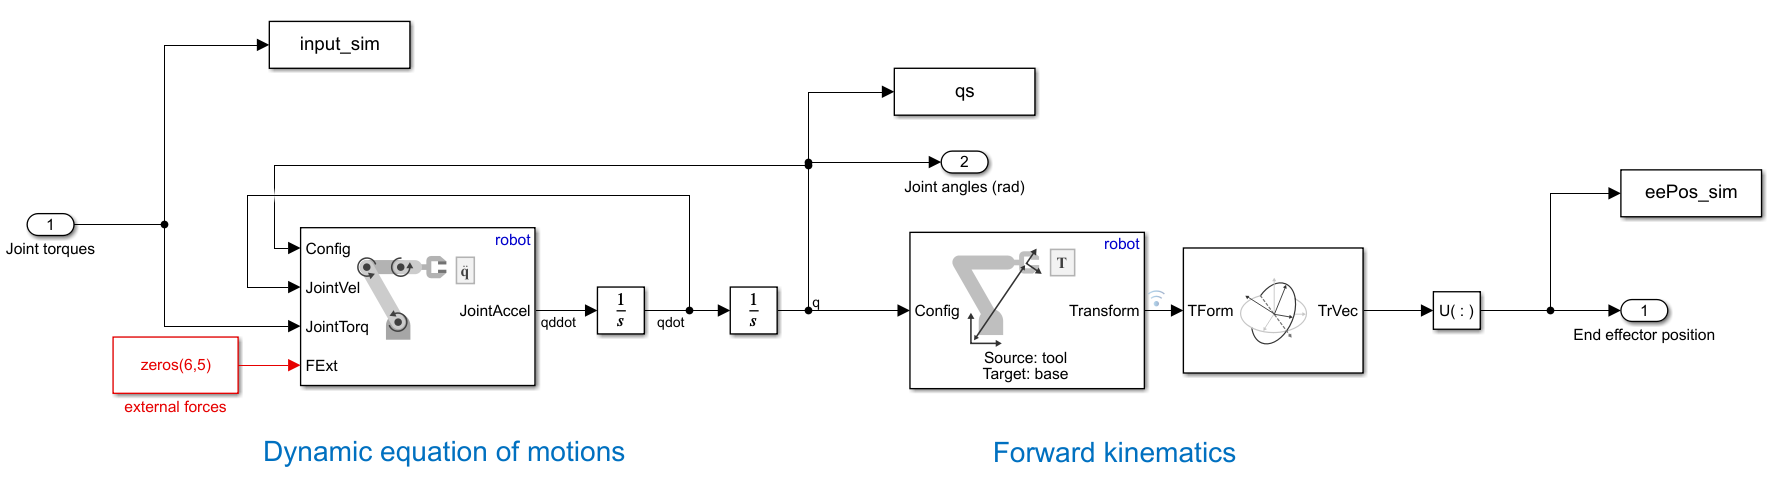
\includegraphics[width=8cm]{./fig/FDK.png}
	\caption{Forward dynamics and kinematics}
	\label{F 5.7}
\end{figure}


\subsection{PID design}



\begin{figure}[htbp]
	\centering
	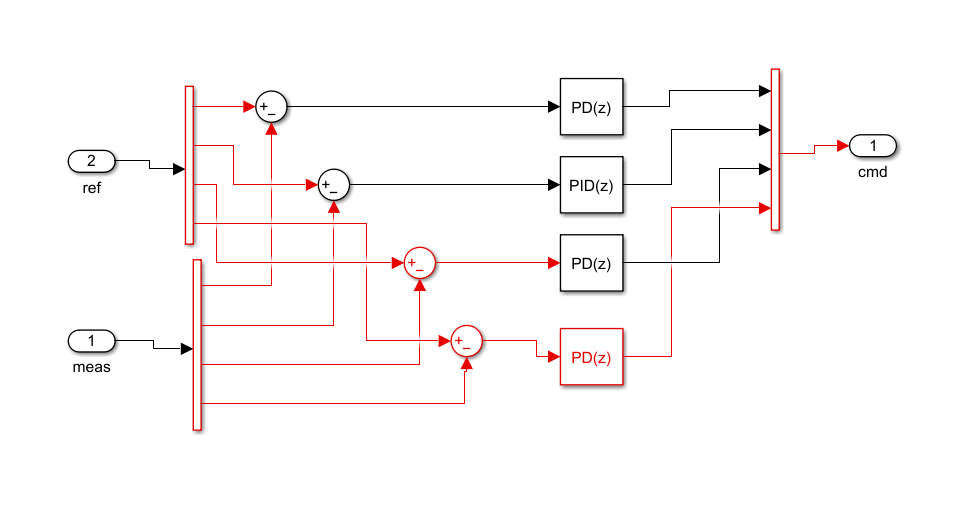
\includegraphics[width=10cm]{./fig/PID.png}
	\caption{PID part}
	\label{F 5.8}
\end{figure}

In the PID control module,as shown in \autoref{F 5.8}, we subtract the desired data from the actual data to obtain the error value, which is then used for PID calculation. We noticed that joints 1, 3, and 4 only use PD controllers because these three joints require a fast response speed and low overshoot, and have lower requirements for steady-state error. For joint 2, which uses a PID controller, it is sensitive to steady-state error due to its rotation around the y-axis. Although there may be difficulty in tuning, we successfully completed the debugging process.


\subsection{Results}

Finally, as shown in \autoref{F 5.9} set the end effector positions and the desired end effector positoins as the input, draw the plot with their x y z positions followed by the time respectively.

\begin{figure}[htbp]
	\centering
	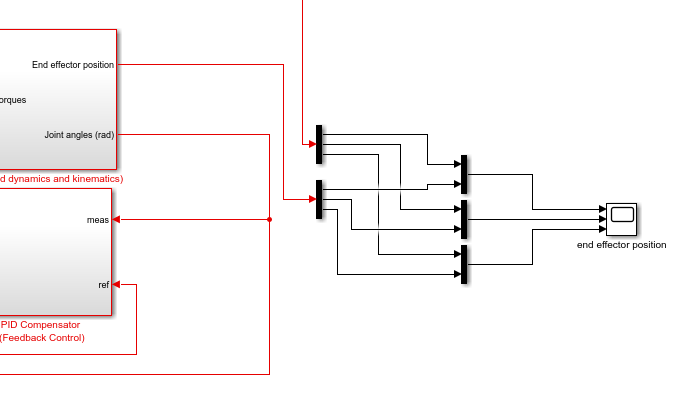
\includegraphics[width=7cm]{./fig/re.png}
	\caption{Export figure part}
	\label{F 5.9}
\end{figure}


\subsubsection*{Input torque}


As shown in \autoref{F 5.10}, this is the torque figure of each joint required for the robot during operation. By observing the figure, it can be found that, except for the initial instability during startup, we only need less than $30N\cdot m$ of torque to drive the robot to complete the welding task.

\begin{figure}[htbp]
	\centering
	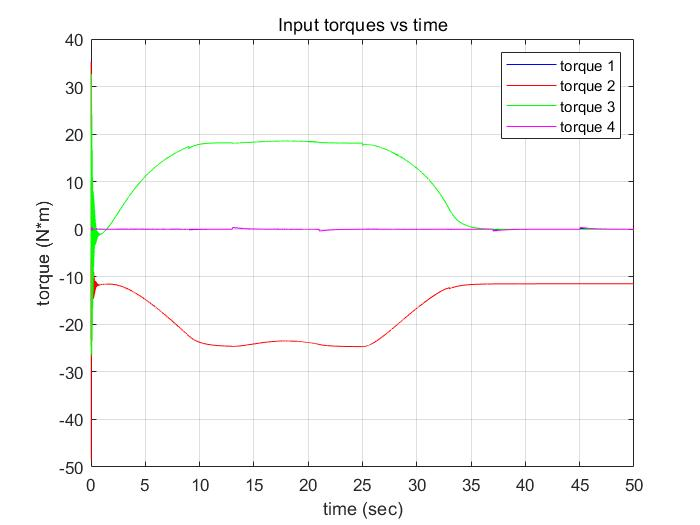
\includegraphics[width=10cm]{./fig/3.jpg}
	\caption{Torque vs Time}
	\label{F 5.10}
\end{figure}

\subsubsection*{Joint angle}




\begin{figure}[htbp]
	\centering
	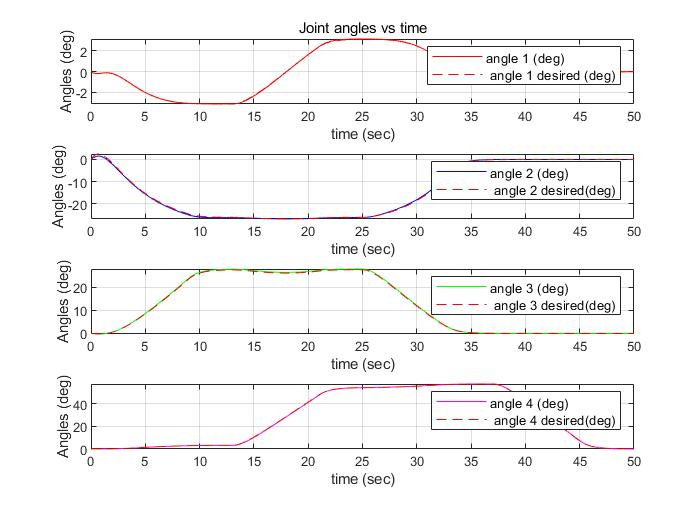
\includegraphics[width=8cm]{./fig/4.jpg}
	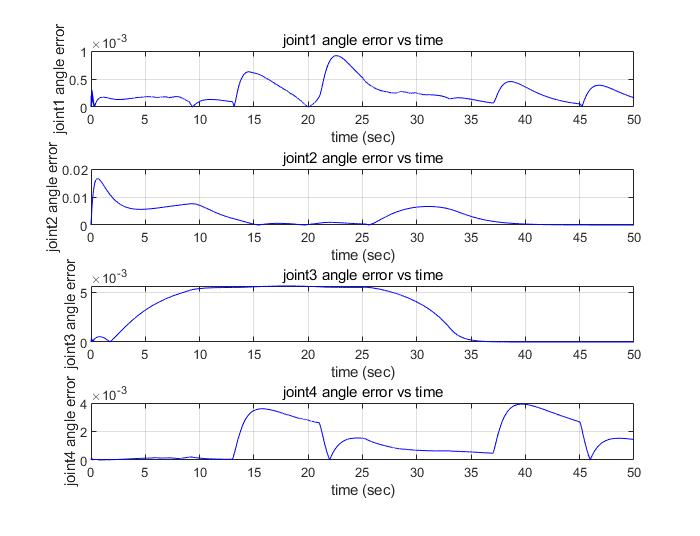
\includegraphics[width=8cm]{./fig/7.jpg}
	\caption{Joint angles vs Time}
	\label{F 5.11}
\end{figure}

As we can see in \autoref{F 5.11}, the error of joint1 angle does not exceed the limit of $10^{-3}$, but it fluctuates throughout the process;
The error of joint2 angle is the largest, and it nearly reaches 0.02, the error tends to be stable except for large fluctuations at the peak throughout the process;
Both the maximum error of joint3 angle and joint4 angle are below $5*10^{-3}$, but joint3 angle error are steady increase to the maximum error, and remain stable on the maximum angle error; as for joint4 angle, there is almost no error in the first ten seconds, and there is always a period of stability after the changes of the error.
Overall, the errors are small and will not have a significant impact on the operation of the robot.

\subsubsection*{End Effector Position}


As we can see in \autoref{F 5.12}, the maximum error in end effector position on the x and z axes is below 0.05, while the maximum error on the y axis is slightly over 0.10. The errors in the x and z axes fluctuate simultaneously, while the error in the y axis gradually increases as the errors in the former axes begin to decrease. There is a small amount of error throughout the entire process, but it is not significant. It has almost no impact in reality.

\begin{figure}[htbp]
	\centering
	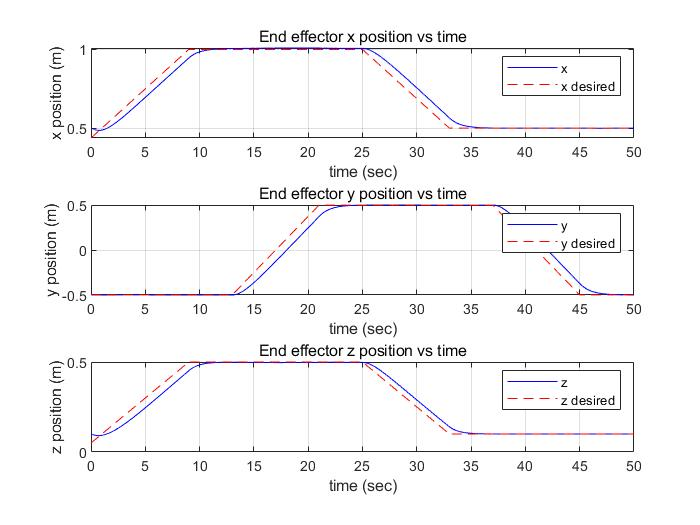
\includegraphics[width=8cm]{./fig/5.jpg}
	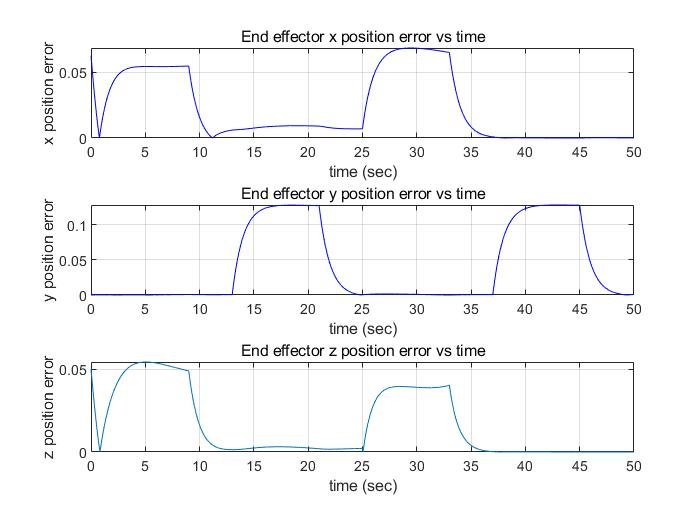
\includegraphics[width=8cm]{./fig/6.jpg}
	\caption{End Effector Position vs Time}
	\label{F 5.12}
\end{figure}

\newpage